\documentclass[a4paper,12pt]{report}
\usepackage{float}
\usepackage{graphicx}
\usepackage{hyperref}
\usepackage{url}
\setcounter{section}{0}
\renewcommand\thesection{\arabic{section}}

\begin{document}

\begin{center}
    \Huge \textbf{Internship Report on Task 3 (Data Cleaning and Insight Generation from Survey)} \\
    \vspace{0.5cm}
    \Large Asmaa Nasr \\
    \vspace{0.5cm}
    \Large \today
\end{center}

\section{Introduction}

This report presents an analysis of the Kaggle Data Science Survey dataset (2017–2021)\cite{b1}. 
The objective of this task was to clean real-world survey data, handle categorical variables, and extract meaningful insights regarding respondent demographics, professional roles, programming preferences, and salary distribution.

\section{Problem / Task Details}

The main objectives were:

\begin{itemize}
    \item Perform data cleaning and remove duplicate entries.
    \item Handle missing and inconsistent values.
    \item Encode categorical variables.
    \item Analyze respondent behavior and professional characteristics.
    \item Create visual summaries of top insights.
\end{itemize}

\section{Dataset Details}

Key variables analyzed:

\begin{itemize}
    \item Country (q3)
    \item Job Title (q5)
    \item Experience (q6)
    \item Programming Languages (q7)
    \item Salary Range (q25)
\end{itemize}

\subsection*{Top 5 Job Titles}

\begin{figure}[H]
\centering
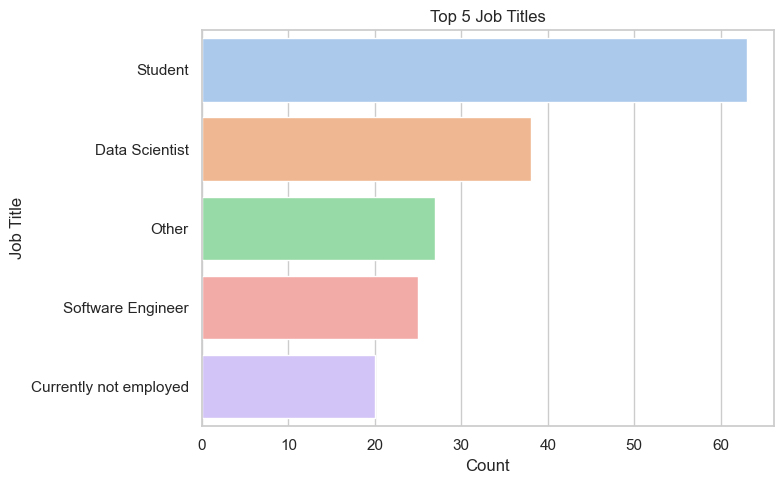
\includegraphics[width=0.9\textwidth]{top_5_jobs.png}
\caption{Top 5 Job Titles of Survey Respondents}
\end{figure}

\subsection*{Top 5 Countries}

\begin{figure}[H]
\centering
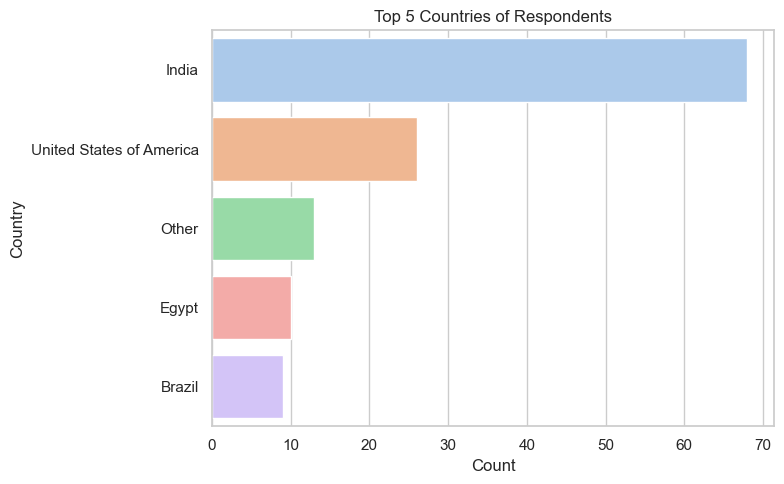
\includegraphics[width=0.9\textwidth]{top_5_countries.png}
\caption{Top 5 Countries of Respondents}
\end{figure}

\subsection*{Experience Distribution}

\begin{figure}[H]
\centering
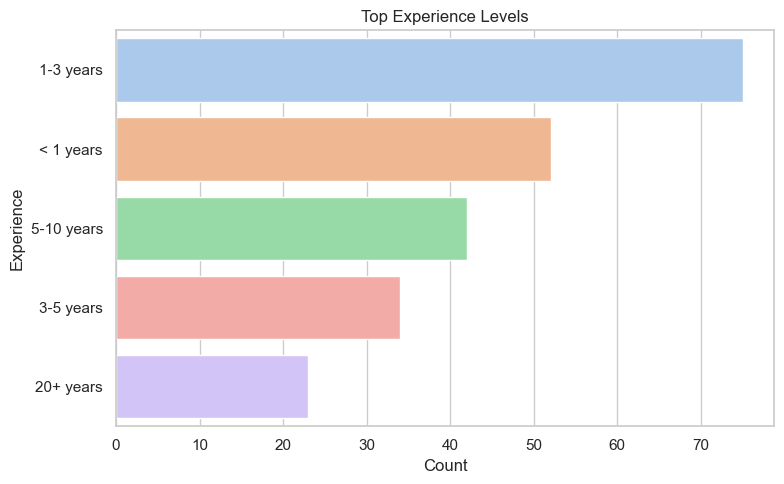
\includegraphics[width=0.9\textwidth]{top_experience.png}
\caption{Experience Level Distribution}
\end{figure}

\subsection*{Top 5 Programming Languages}

\begin{figure}[H]
\centering
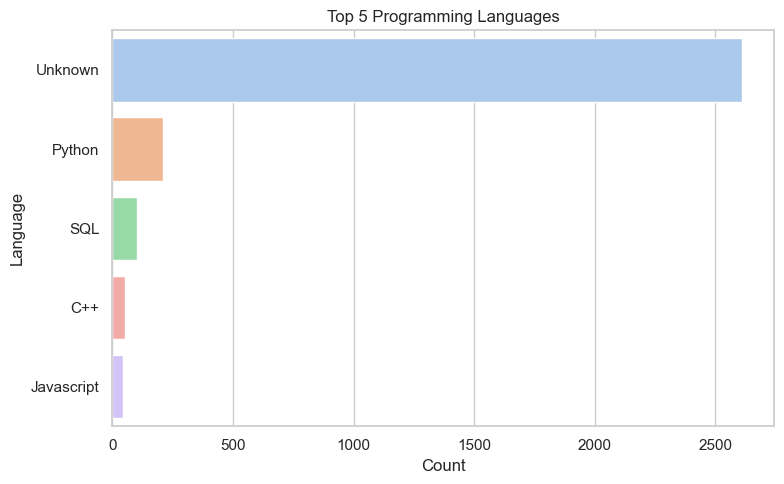
\includegraphics[width=0.9\textwidth]{top_5_languages.png}
\caption{Top 5 Programming Languages Used}
\end{figure}

\subsection*{Top Salary Ranges}

\begin{figure}[H]
\centering
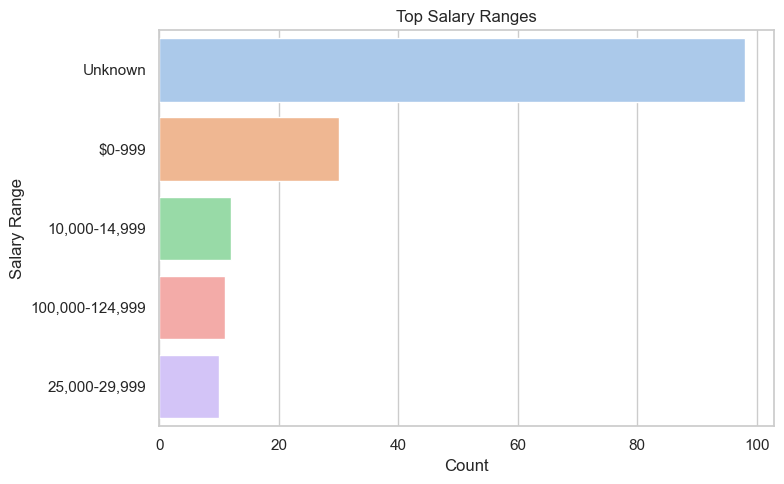
\includegraphics[width=0.9\textwidth]{top_salary.png}
\caption{Top Salary Ranges of Respondents}
\end{figure}

\section{Conclusion}

The analysis demonstrates that Python dominates the data science ecosystem, and a significant proportion of respondents are early-career professionals or students. 
The survey responses are geographically concentrated in a few major countries, and salary distribution is primarily centered around mid-level income ranges.

This task highlights the importance of proper data cleaning, categorical handling, and structured exploratory data analysis when working with real-world datasets.

\begin{thebibliography}{99}

\bibitem{b1} Kaggle Survey Dataset (2017--2021), Kaggle Inc. Available at: \url{https://www.kaggle.com}

\end{thebibliography}

\end{document}
